\begin{figure*}[t]
\centering
\ifbilingual
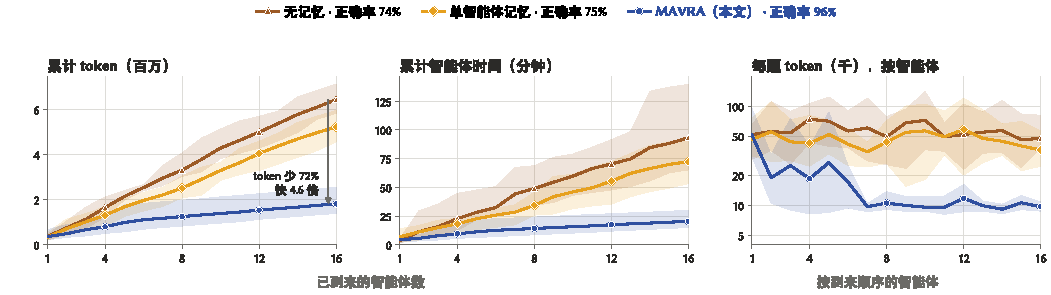
\includegraphics[width=\textwidth]{figures/population-zh}
\else
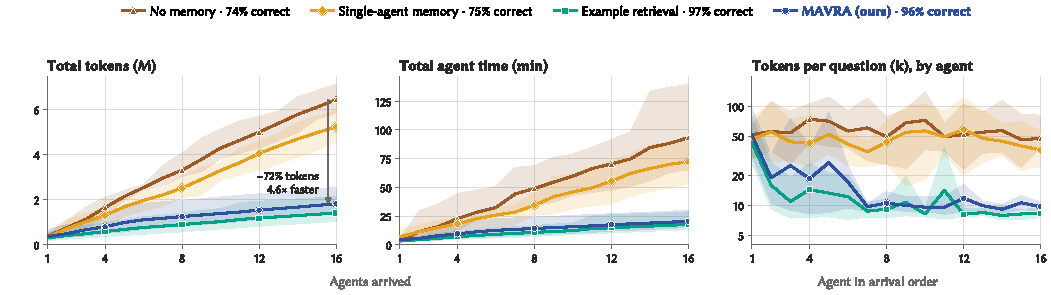
\includegraphics[width=\textwidth]{figures/population}
\fi
\caption{\bt{What \PpAgents\ agents arriving at one TPC-DS database pay, by memory design. Left and middle: total tokens (including learning) and total agent time of the first $N$ agents. Right: tokens per question of each agent in arrival order (log scale): with \system\ the first agents pay for learning and every later agent reuses. Lines are means over \PpRuns\ runs, bands span the runs; the legend gives each method's accuracy.}{\PpAgents\ 个智能体陆续使用同一 TPC-DS 数据库时，不同记忆设计下的代价。左、中：前 $N$ 个智能体的累计 token（含学习）与累计智能体时间。右：按到来顺序每个智能体每题的 token（对数坐标）：使用 \system\ 时，最先到来的智能体为学习付出代价，之后每个智能体都复用。线为 \PpRuns\ 次运行的均值，色带覆盖各次运行；图例给出各方法的正确率。}}
\label{fig:population}
\Description{Three line charts for no memory, single-agent memory, and MAVRA. Left: total tokens in millions against the number of agents that have arrived, 1 to 16. Middle: total agent time in minutes. Right: tokens per question of each agent in arrival order on a log scale; no memory stays around 50 thousand, single-agent memory declines slowly, and MAVRA drops to about 10 thousand after the first two or three agents. Values are filled in from the population study.}
\end{figure*}
